% -*- coding: utf-8 -*-
% vim: autoindent expandtab tabstop=4 sw=4 sts=4 filetype=tex
% vim: spelllang=de spell
% chktex-file 27 - disable warning about missing include files

\section{Logische Architektur}
\label{sec:logical-architecture}

Die logische Architektur zeigt das Gesamtbild der Software-Klassen in Form von
Paketen (bzw. Namespaces), Subsystemen und Layern~\cite[S. 199]{larman_applying_2004}.
Bei Layern handelt es sich um eine grobe Gruppierung von Klassen, Paketen oder
Subsystemen, welche zusammenhängen~\cite[S. 199]{larman_applying_2004}.

Eine strikt abgestufte (strict layered) Architektur sieht vor, dass ein Layer
nur Services beziehungsweise Schnittstellen der darunterliegenden Schicht
aufruft~\cite[S. 200]{larman_applying_2004}.

Da dies in der Praxis je nach Fall der Anwendung jedoch schwer umzusetzen ist,
wird häufig auch von einer locker abgestuften (relaxed layered) Architektur
gesprochen~\cite[S.  200]{larman_applying_2004}. Diese ermöglicht es, dass
höhere Stufen ohne Weiteres mit wesentlich tieferen Stufen kommunizieren. Eine
solche Architektur wird hier angestrebt.\\
Die Verwendung dieses Design-Musters reduziert Kupplung (coupling) sowie
Abhängigkeiten, erhöht Kohäsion und Klarheit~\cite[S.
204]{larman_applying_2004}.

Um dies auch hinsichtlich der grafischen Benutzeroberfläche zu gewährleisten,
wurde zudem das Prinzip der Trennung von Modellen und Ansichten (model-view
separation principle) angewendet. Dieses sagt aus, dass Modelle beziehungsweise
Objekte einer Domäne kein direktes Wissen über Objekte der grafischen
Benutzeroberfläche haben sollen~\cite[S.  209]{larman_applying_2004}.\\
Die Trennung von Modellen und Ansichten führt zu oder unterstützt kohäsive
(geschlossene) Modelle, welche auf die Prozesse der Domäne fokussiert sind
anstatt auf die grafische Benutzeroberfläche~\cite[S.
210]{larman_applying_2004}.

Da diese Trennung doch sehr strikt ist, kann das Observer-Muster als weniger
strikte Version angesehen werden~\cite[S. 210]{larman_applying_2004}. Ein
Domänen-Objekt sendet Nachrichten zu reinen Schnittstellen von Objekten der
grafischen Benutzeroberfläche. Somit weiss das Domänen-Objekt nicht, dass es
sich bei dem angesprochenen Objekt um ein Objekt der grafischen
Benutzeroberfläche handelt~\cite[S. 210]{larman_applying_2004}.
Dieser Schritt wurde in dieser Version jedoch nicht umgesetzt. Es wird sich in
der darauffolgenden Projektarbeit zeigen, ob dies nötig ist.

Als zusätzliche Abstraktion wurden noch Controller eingeführt. Controller
stellen Workflow-Objekte der Applikationsschicht dar~\cite[S.
209]{larman_applying_2004}.

Die logische Architektur umfasst folgende Elemente:
\begin{itemize}
    \item~\textbf{UI}\\
        Alle Elemente der grafischen Benutzeroberfläche.

    \item~\textbf{Application}\\
        Controller / Workflow-Objekte.

    \item~\textbf{Domain}\\
        Modelle / Applikationslogik.

    \item~\textbf{Technical services}\\
        Technische Infrastruktur wie Grafik, Erzeugung von Fenstern etc.

    \item~\textbf{Foundation}\\
        Grundlegende Elemente, low-level technical services wie Timer, Array
        oder andere Datenklassen.
\end{itemize}

Sowohl für den Player als auch für den Editor ist dieselbe logische Architektur
vorgesehen. Ein grosser Teil der Pakete überschneidet sich bei beiden
Komponenten, da beide dieselbe (Daten-) Struktur nutzen. Beim Paket-Diagramm
des Players wurde dies jedoch der Übersicht halber, sowie zur Vermeidung von
unnötiger Redundanz weggelassen. Auch hier gilt wiederum, dass essentielle
Konzepte beziehungsweise Objekte fehlen. Diese werden während den Iterationen
der darauffolgenden Projektarbeit erarbeitet. Es sind jedoch bereits mehr
Elemente angedeutet, als in den vorherigen Diagrammen.

Abbildung~\ref{fig:package-diagram:layers} zeigt die verschiedenen Schichten
als Übersicht. Abbildung~\ref{fig:package-diagram:player} zeigt das Paket-Diagramm des
Players, Abbildung~\ref{fig:package-diagram:editor} dies des Editors.
Blau-graue Elemente stellen dabei selbst entwickelte Pakete, violette Elemente
externe Pakete von Drittpersonen dar.

\begin{figure}[H]
    \centering
    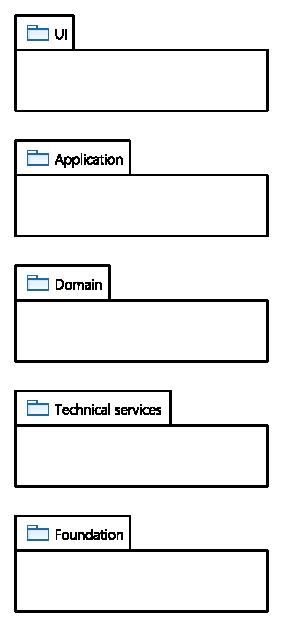
\includegraphics[width=0.3\textwidth]{img/layers.PDF}
    \caption{Paket-Diagramm der
        Player-Applikation}\label{fig:package-diagram:layers}
\end{figure}

\begin{figure}[H]
    \centering
    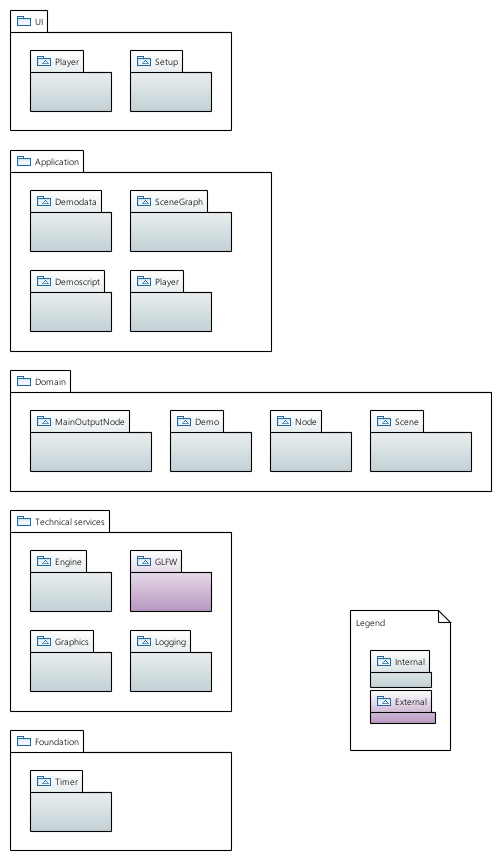
\includegraphics[width=0.9\textwidth]{img/player_package_diagram.PNG}
    \caption{Paket-Diagramm der Player-Applikation}\label{fig:package-diagram:player}
\end{figure}

\begin{figure}[H]
    \centering
    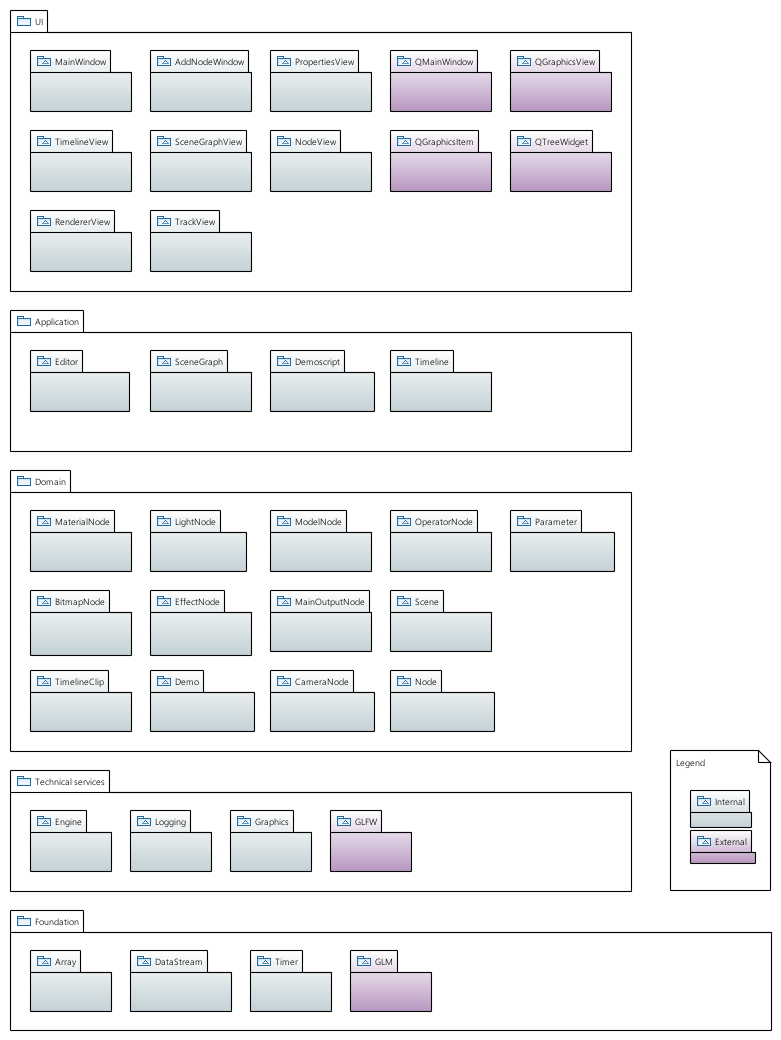
\includegraphics[width=1.0\textwidth]{img/editor_package_diagram.PNG}
    \caption{Paket-Diagramm der Editor-Applikation}\label{fig:package-diagram:editor}
\end{figure}
